\documentclass{article}
\usepackage{graphicx}
\usepackage{listings}
\usepackage{color}
\usepackage{amsmath}
\usepackage{amsfonts}
\usepackage{bm}
\usepackage[utf8]{inputenc}

\title{Modelli di crescita della popolazione\\
	Corso di LSMC, a.a. 2017-2018}
\author{Davide Gori\\
	550282}


\definecolor{backcolour}{rgb}{0.95,0.95,0.92}
\definecolor{gray}{rgb}{0.5,0.5,0.5}
\lstset{basicstyle=\ttfamily\small,
	columns=fullflexible,
	numbers=left,
	numberstyle=\tiny\ttfamily\color{gray},
	backgroundcolor=\color{backcolour},
	tabsize=4,
	language=Octave
}


\begin{document}
	\maketitle
	\section{Prima sperimentazione: Lotka-Volterra}
	Il modello di Lotka-Volterra che descrive la dinamica delle due popolazioni si scrive come segue:
		\begin{equation}
	\begin{cases}
	y_1' = y_1 \cdot \gamma_1 \cdot (1-\frac{y_1}{k_1}-\frac{y_2}{h_12}) \\
	y_2' = y_2 \cdot \Gamma_2 \cdot (1-\frac{y_2}{k_2}+\frac{y_1}{h_21}) \\
	\end{cases}
	\end{equation}
	dove $y_1(t)$ ed $y_2(t)$ indicano il volume in cc (centimetri cubi) occupato dalla prima e seconda popolazione di lieviti al tempo $t$ (misurato in ore). I valori calcolati da Gause sono i seguenti:\\
	$\gamma_1 = 0.21827$, $k_1 = 13$, $h_12 = 3.71429$; $\gamma_2 = 0.06069$, $k_2 = 5.8$, $h_21 = 13.2118$.\\
	Utilizzando la routine {\tt ode45} risolverò il sistema con i seguenti dati iniziali: $y_1(0) = 0.5$, $y_2(0) = 0.3$, sull'intervallo $\left[0, 300\right]$. Disegnerò sulla stessa figura i grafici della densità di popolazione.\\
	Inoltre, fissato $y_2(0) = 0.5$, analizzerò i tre casi:\\
	$y_1(0) = 0.5$, $y_2(0) = 0.1$, $y_3(0) = 10$.
	
	\subsection{L'implementazione}
	l'equazione è ({\tt fun}):
	\begin{equation}
	\begin{cases}
	y'(1) = y(1) \cdot 0.21827 \cdot (1-\frac{y(1)}{13}-\frac{y(2)}{3.71429}) \\
	y'(2) = y(2) \cdot 0.06069 \cdot (1-\frac{y(2)}{5.8}+\frac{y(1)}{13.2118}) \\
	\end{cases}
	\end{equation}
	\subsection{Il codice}
	Questo è lo script che realizza la prima sperimentazione:
	\lstinputlisting{LabSper_4_1_1.m}
	Dove {\tt fun} è la seguente:
	\lstinputlisting{fun.m}
	Questo è lo script che realizza la seconda sperimentazione:
	\lstinputlisting{LabSper_4_1_2.m}
	Dove {\tt fun} è la seguente:
	\lstinputlisting{fun.m}
	
	\subsection{Risultati}
	Riportiamo il grafico in output.\\
	\begin{figure}[htp!]
		\centering 
		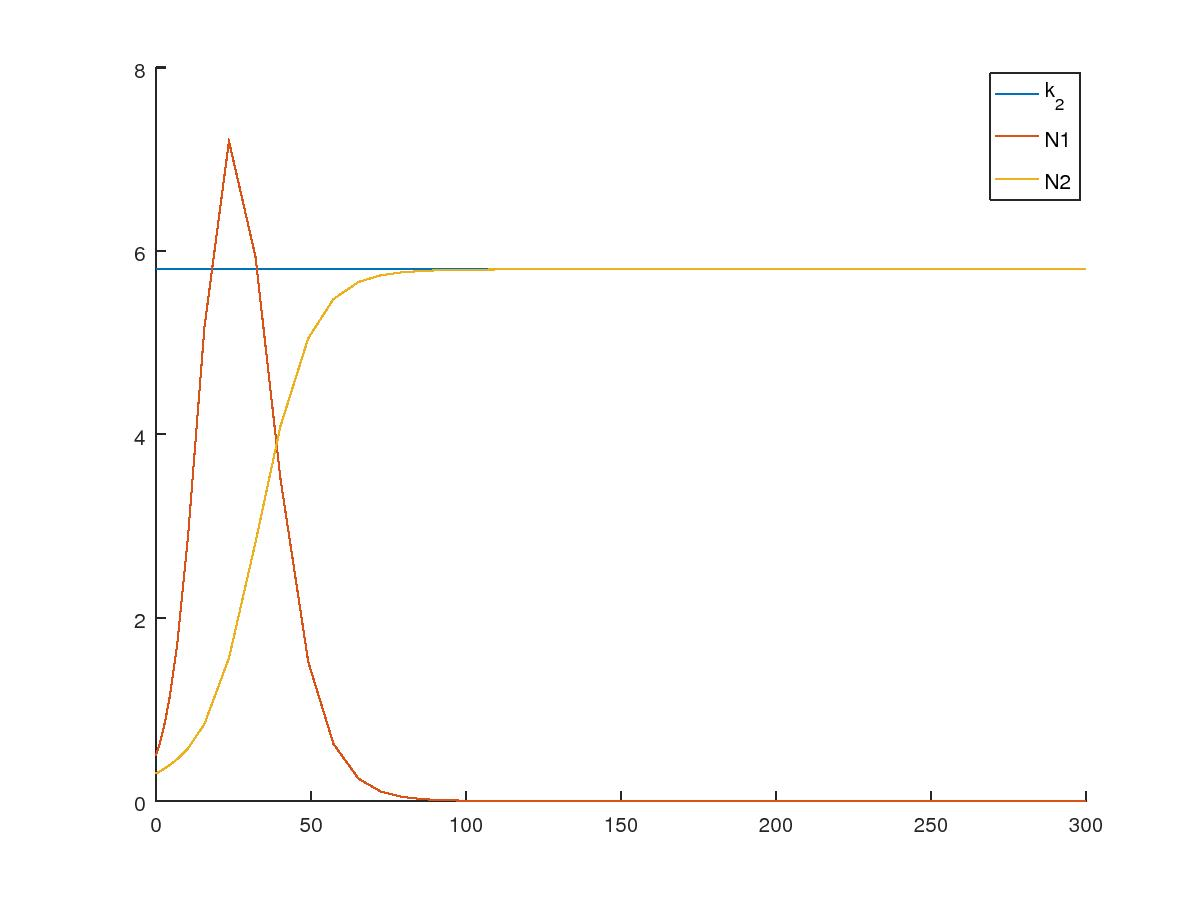
\includegraphics[width=0.5\textwidth]{4_1_1.jpeg}
	\end{figure}
	\newpage
	Riportiamo il grafico in output.\\
	In tutti e tre i casi si verifica che dopo un transiente, circa della stessa durata per le tre poplazioni, la specie N2 si stabilizza a 5.8 e quella N2 si estingue.\\
	\begin{figure}[htp!]
	\centering 
	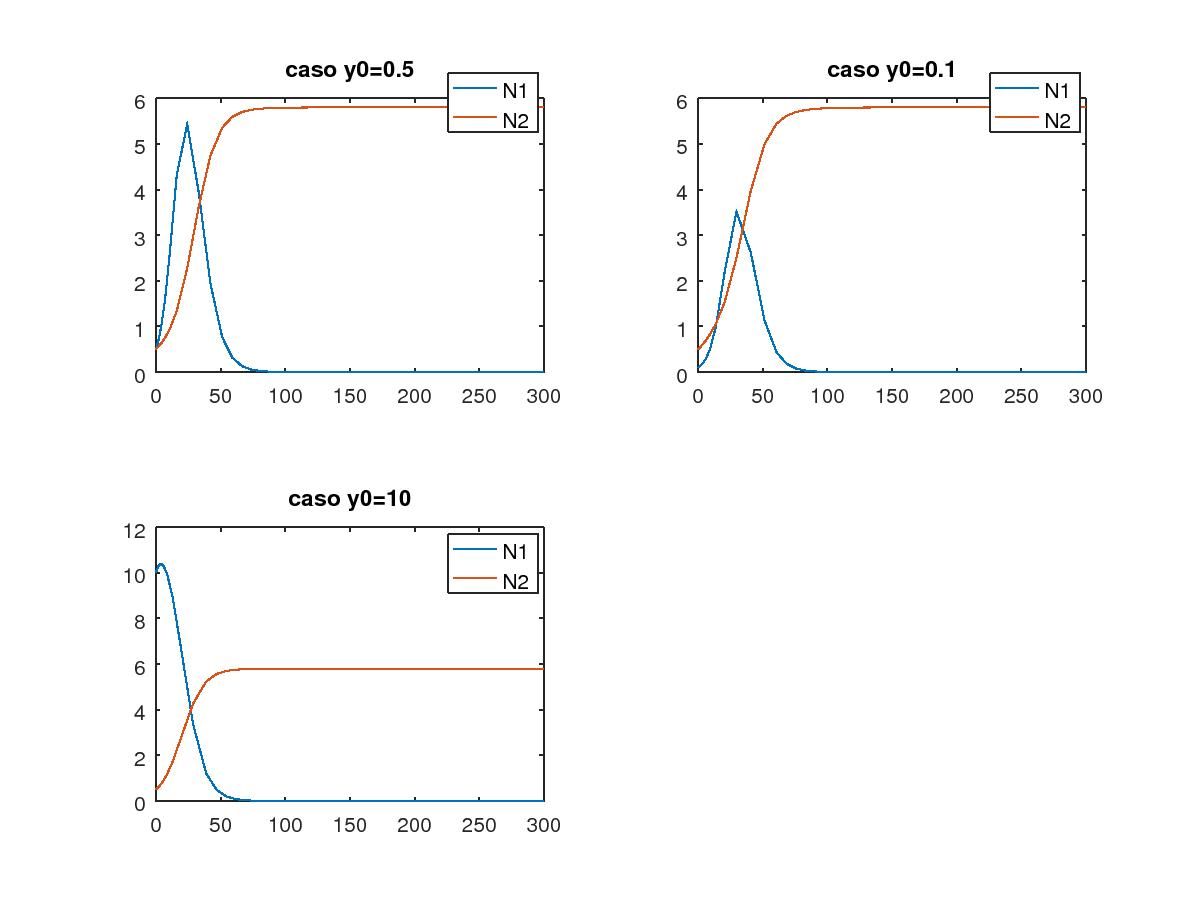
\includegraphics[width=\textwidth]{4_1_2.jpeg}
	\end{figure}

	\section{Seconda sperimentazione: Lotka-Volterra V2}
	Il modello di Lotka-Volterra che descrive la dinamica delle due popolazioni si scrive come segue:
	\begin{equation}
	\begin{cases}
	y_1' = y_1 \cdot \gamma_1 \cdot (1-\frac{y_1}{k_1}-\frac{y_2}{h_12}) \\
	y_2' = y_2 \cdot \Gamma_2 \cdot (1-\frac{y_2}{k_2}+\frac{y_1}{h_21}) \\
	\end{cases}
	\end{equation}
	Utilizzeremo il metodo di Runge-Kutta classico con i seguenti parametri: $\alpha = 2$, $\beta = 0$, $\gamma = 0.001$; $\hat{\alpha} = 1$, $\hat{\beta} = 0.001$.\\
	supponendo che le densità iniziali siano le seguenti:
	\begin{itemize}
		\item $y_1(0) = 300$, $y_2(0) = 150$.
		\item $y_1(0) = 15$, $y_2(0) = 22$.
	\end{itemize}
	
	\subsection{Il codice}
	Questo è lo script che realizza la sperimentazione:
	\lstinputlisting{LabSper_4_2.m}
	Dove {\tt fun1} è la seguente:
	\lstinputlisting{fun1.m}
	
	\subsection{Risultati}
	Riportiamo il grafico in output.\\
	\begin{figure}[htp!]
		\centering 
		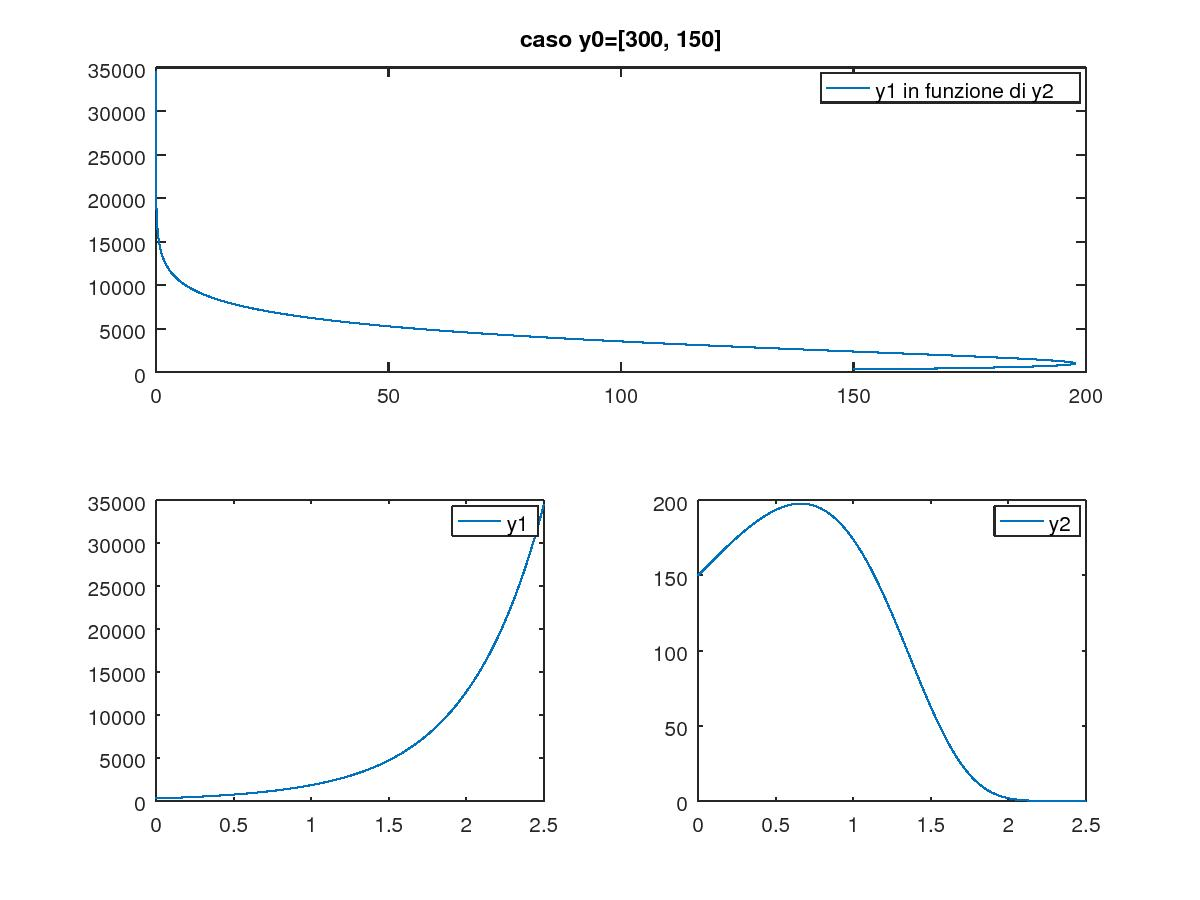
\includegraphics[width=\textwidth]{4_2_a.jpeg}
	\end{figure}
	\newpage
	Riportiamo il grafico in output.\\
	
	\begin{figure}[htp!]
		\centering 
		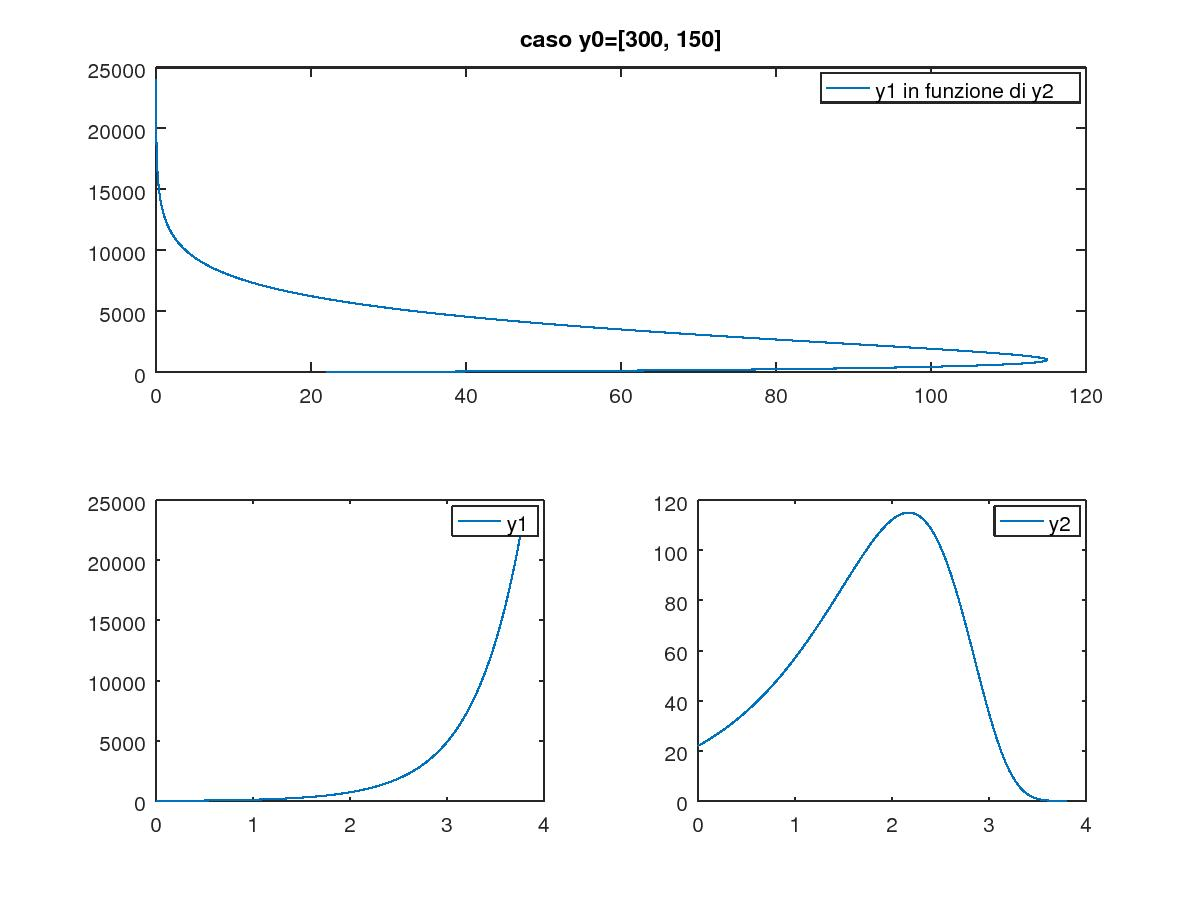
\includegraphics[width=\textwidth]{4_2_b.jpeg}
	\end{figure}
	
	Visti i coefficienti dell'equazione differenziale ci si aspetta una crescita pressoché esponenziale (per y1), in effetti questa previsione è rispettata.\\
	I valori scelti per h e tmax sono i seguenti:
	\begin{itemize}
		\item modello $y(0)=[300, 150]$, $h=0.0001$, $tmax=2.5$
		\item modello $y(0)=[15, 22]$, $h=0.0001$, $tmax=3.8$
	\end{itemize}
	è possibile aumentare h di un fattore 10 a seconda delle prestazioni del calcolatore, il risultato è pressapoco lo stesso.
	
	\section{Terza sperimentazione: Lotka-Volterra V3}
	Il modello di Lotka-Volterra che descrive la dinamica delle due popolazioni si scrive come segue:
	\begin{equation}
	\begin{cases}
	G' = G (0.405-0.81 L) \\
	L'= L (-1.5+0.125 G)\\
	\end{cases}
	\end{equation}
	Sapendo $G(1975) = 7.7$ e $L(1975) = 0.5$. Utilizziamo la routine {\tt ode45}, sull'intervallo $[0, T]$ per $T = 10$ e $T = 25$.\\
	Nel primo caso, rappresenteremo come varia il numero dei predatori in funzione del numero di prede, mentre nel secondo plotteremo il numero delle prede ed il numero dei predatori rispetto al tempo.	
	\subsection{Implementazione}
	\begin{equation}
		\begin{cases}
			y_1' = y_1 (0.405-0.81 y_2) \\
			y_2'= y_2 (-1.5+0.125 y_1)\\
		\end{cases}
	\end{equation}
	con $G=y(1)$ e $L=y(2)$.\\
	Essendo l'equazione autonoma supponiamo $T_0=0$.
	
	\subsection{Il codice}
	Questo è lo script che realizza la sperimentazione:
	\lstinputlisting{LabSper_4_3.m}
	Dove {\tt fun2} è la seguente:
	\lstinputlisting{fun2.m}
	
	\subsection{Risultati}
	Riportiamo il grafico in output.\\
	\begin{figure}[htp!]
		\centering 
		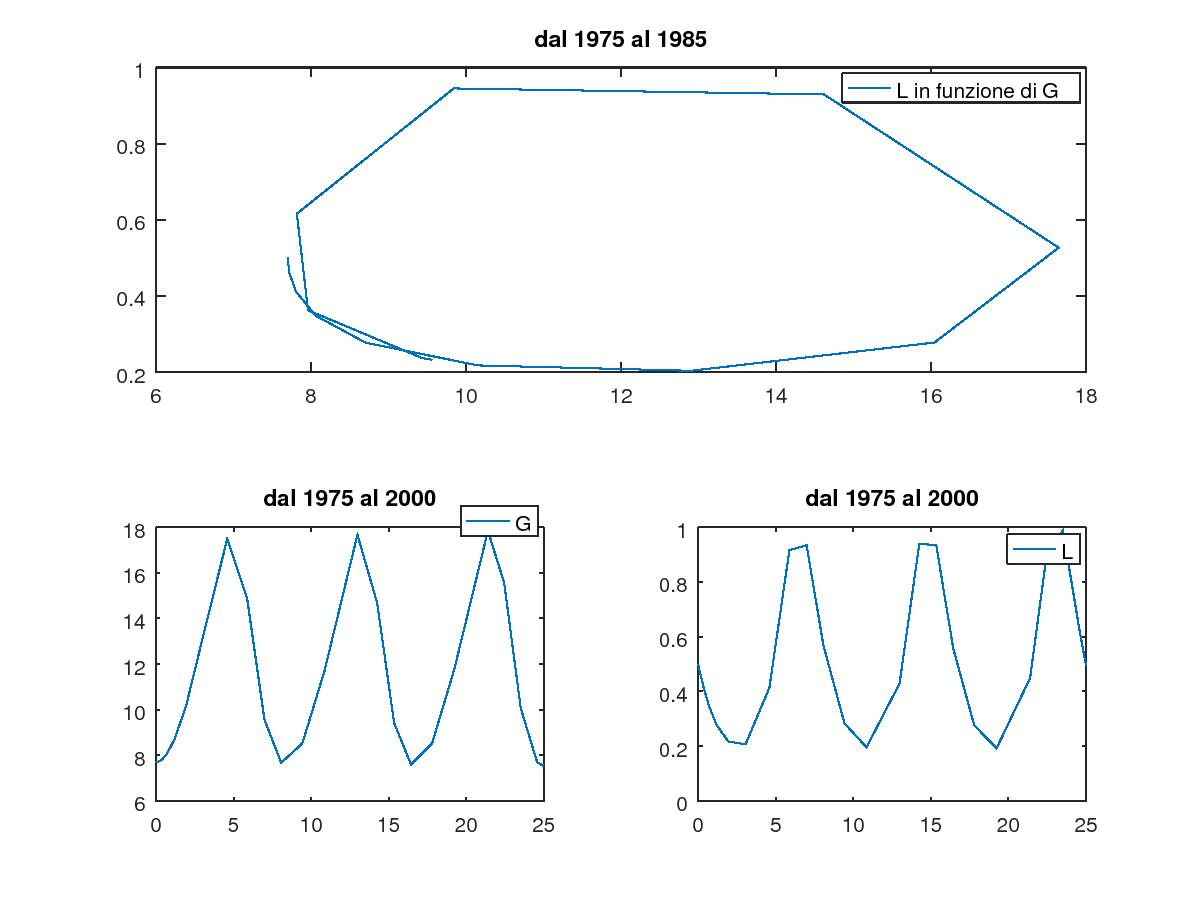
\includegraphics[width=\textwidth]{4_3.jpeg}
	\end{figure}

	Si può notare che l'andamento di L e G é quasi periodico.
	
	\section{Quarta sperimentazione: modellizzare una malattia}
	Supponiamo che una popolazione di $N$ individui si ainfettata da una malattia inguaribile e non mortale, indicando con $S(t)$ il numero di persone sane e con $I(t)$ quelle infette, si ha che $S(t)+I(t)=N$. Determinerò un modello matematico che descrive la situazione e testerò questo su un esempio dato.	
	\subsection{Implementazione}
	Supponiamo $r \geq 0$ il tasso di rischio di infezione, otteniamo il seguente modello:
	\begin{equation}
	\begin{cases}
	I(t) = r I(t)(N-I(t))\\
	I(0)=I_0\\
	\end{cases}
	\end{equation}
	Il modello implementato è il modello SIR con parametro $\beta=0$, notando che $I+S=N$.
	Per far si che il modello abbia senso fisico occorre che: $I(0)$ sia intero e appartenente all'intervallo $\left[0, N\right]$. Essendo l'equazione autonoma supponiamo $t_0=0$.
	
	Proviamo a implementare un caso reale con i seguenti dati:\\
	$N=1000$, $r=0.0001$ e $I(0)=1$ 
	\subsection{Il codice}
	Questo è lo script che realizza la sperimentazione:
	\lstinputlisting{LabSper_4_4.m}
	Dove {\tt fun3} è la seguente:
	\lstinputlisting{fun3.m}
	
	\subsection{Risultati}
	Riportiamo il grafico in output.\\
	\begin{figure}[htp!]
		\centering 
		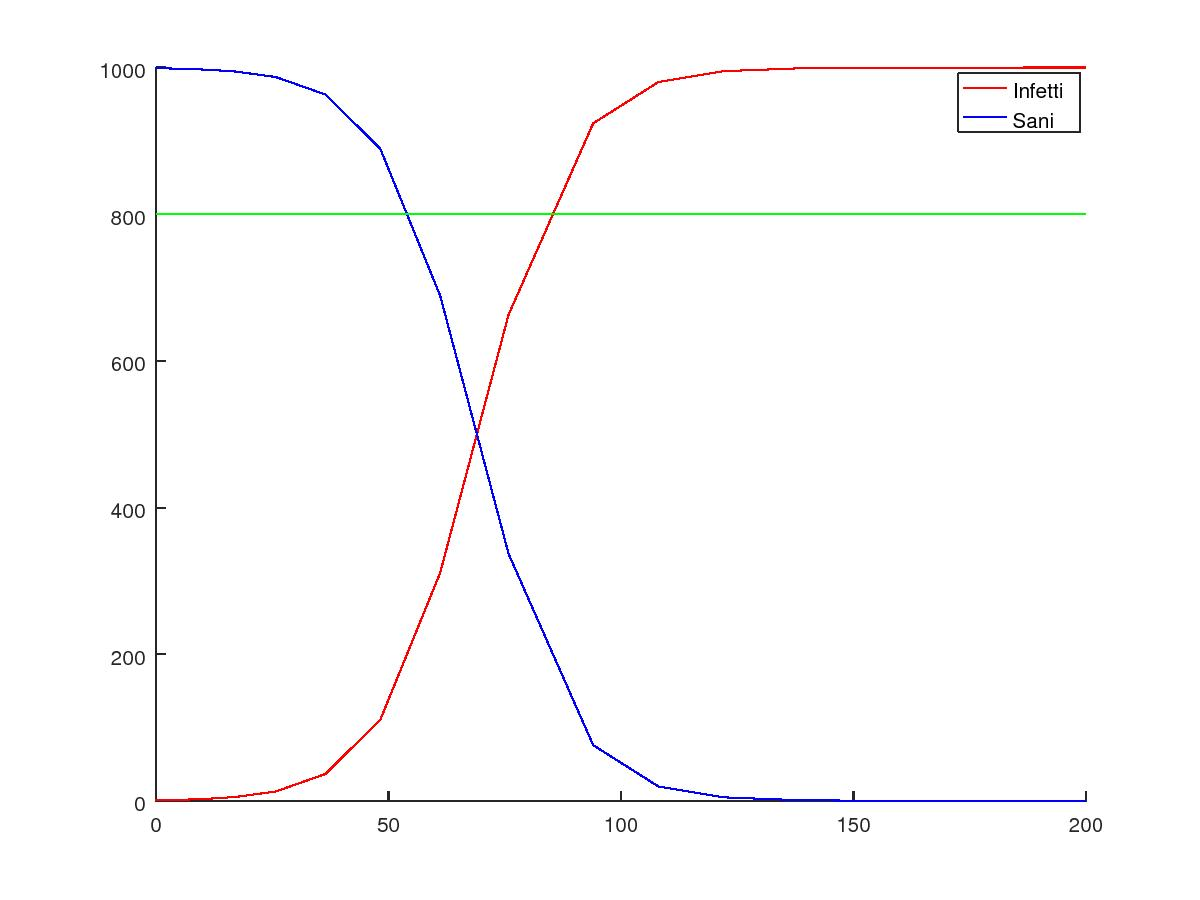
\includegraphics[width=\textwidth]{4_4.jpeg}
	\end{figure}
	
	Graficamente si vede che l'$80\%$ viene superato circa all'80-esimo giorno di diffusione della malattia.
\end{document}